\chapter{Mengenal Kecerdasan Buatan dan ScikitLearn}

\section{Teori}

\subsection{Kecerdasan Buatan}
RESUME 1

\paragraph{Definisi}\hspace{0pt} \par
Kecerdasan Buatan adalah kemampuan komputer digital atau robot yang dikendalikan komputer untuk melakukan tugas yang umumnya dikaitkan dengan sesuatu yang cerdas. Istilah ini sering diterapkan pada proyek pengembangan sistem yang diberkahi dengan karakteristik proses intelektual manusia, seperti kemampuan untuk berpikir, menemukan makna, menggeneralisasi, atau belajar dari pengalaman masa lalu.

\paragraph{Sejarah Singkat}\hspace{0pt}\par
Pada awal 50-an, studi tentang "mesin bepikir" memiliki berbagai nama seperti cybernetics, teori automata, dan pemrosesan informasi. Pada tahun 1956, para ilmuwan jenius seperti Alan Turing, Norbert Wiener, Claude Shannon dan Warren McCullough telah bekerja secara independen di bidang cybernetics, matematika, algoritma dan teori jaringan.
Namun, seorang ilmuwan komputer dan kognitif John McCarthy adalah orang yang datang dengan ide untuk bergabung dengan upaya penelitian terpisah ini ke dalam satu bidang yang akan mempelajari topik baru untuk imajinasi manusia yaitu Kecerdasan Buatan. Dia adalah orang yang menciptakan istilah tersebut dan kemudian mendirikan laboratorium Kecerdasan Buatan di MIT dan Stanford.
Pada tahun 1956, McCarthy yang sama mendirikan Konferensi Dartmouth di Hanover, New Hampshire. Peneliti terkemuka dalam teori kompleksitas, simulasi bahasa, hubungan antara keacakan dan pemikiran kreatif, jaringan saraf diundang. Tujuan dari bidang penelitian yang baru dibuat adalah untuk mengembangkan mesin yang dapat mensimulasikan setiap aspek kecerdasan. Itulah sebabnya Konferensi Dartmouth 1956 dianggap sebagai kelahiran Kecerdasan Buatan.
Sejak itu, Kecerdasan Buatan telah hidup melalui dekade kemuliaan dan cemoohan, yang dikenal luas sebagai musim panas dan musim dingin AI. Musim panasnya ditandai dengan optimisme dan dana besar, sedangkan musim dinginnya dihadapkan dengan pemotongan dana, ketidakpercayaan dan pesimisme.

\paragraph{Perkembangan Kecerdasan Buatan}\hspace{0pt} \par
AI Summer 1 [1956-1973]
Konferensi Dartmouth diikuti oleh 17 tahun kemajuan luar biasa. Proyek penelitian yang dilakukan di MIT, universitas di Edinburgh, Stanford dan Carnegie Mellon menerima dana besar-besaran, yang akhirnya membuahkan hasil.
Selama tahun-tahun itulah komputer pemrograman mulai melakukan masalah aljabar, membuktikan teorema geometris, memahami dan menggunakan sintaks dan tata bahasa Inggris. Terlepas dari ditinggalkannya koneksionisme dan terjemahan mesin yang gagal, yang menunda penelitian Natural Language Processing (NLP) selama bertahun-tahun, banyak prestasi dari masa lalu yang membuat sejarah. Berikut ini beberapa di antaranya:
Pelopor pembelajaran mesin, Ray Solomonoff meletakkan dasar-dasar teori matematika AI, memperkenalkan metode Bayesian universal untuk inferensi dan prediksi induktif Thomas Evans menciptakan program ANALOGI heuristik, yang memungkinkan komputer memecahkan masalah geometri-analogi Unimation, perusahaan robotika pertama di dunia, menciptakan robot industri Unimate, yang bekerja pada jalur perakitan mobil General Motors. Joseph Weizenbaum membangun ELIZA - program interaktif yang dapat membawa percakapan dalam bahasa Inggris tentang topik apa pun.Ross Quillian menunjukkan jaring semantik, sedangkan Jaime Carbonell (Sr.) mengembangkan Cendekia - program interaktif untuk instruksi yang dibantu komputer berdasarkan jaring semantik. Edward Feigenbaum dan Julian Feldman menerbitkan Computers and Thought, kumpulan artikel pertama tentang AI.
\subsection{Definisi}
RESUME 2

\paragraph{Supervised Learning}\hspace{0pt}  \par
Supervised Learning adalah tugas pengumpulan data untuk menyimpulkan fungsi dari data pelatihan berlabel. Data pelatihan terdiri dari serangkaian contoh pelatihan. Dalam supervised learningi, setiap contoh adalah pasangan yang terdiri dari objek input (biasanya vektor) dan nilai output yang diinginkan (juga disebut sinyal pengawasan super). Algoritma pembelajaran yang diawasi menganalisis data pelatihan dan menghasilkan fungsi yang disimpulkan, yang dapat digunakan untuk memetakan contoh-contoh baru. Skenario optimal akan memungkinkan algoritma menentukan label kelas dengan benar untuk instance yang tidak terlihat. Ini membutuhkan algoritma pembelajaran untuk menggeneralisasi dari data pelatihan untuk situasi yang tidak terlihat dengan cara yang “masuk akal”.
Supervised Learningi menyediakan algoritma pembelajaran dengan jumlah yang diketahui untuk mendukung penilaian di masa depan. Chatbots, mobil self-driving, program pengenalan wajah, sistem pakar dan robot adalah beberapa sistem yang dapat menggunakan pembelajaran yang diawasi atau tidak diawasi. Supervised Learning sebagian besar terkait dengan AI berbasis pengambilan tetapi mereka juga mungkin mampu menggunakan model pembelajaran generatif.
Data pelatihan untuk pembelajaran yang diawasi mencakup serangkaian contoh dengan subjek input berpasangan dan output yang diinginkan (yang juga disebut sebagai sinyal pengawasan). Dalam pembelajaran yang diawasi untuk pemrosesan gambar, misalnya, sistem AI mungkin dilengkapi dengan gambar berlabel kendaraan dalam kategori seperti mobil dan truk. Setelah jumlah pengamatan yang cukup, sistem harus dapat membedakan antara dan mengkategorikan gambar yang tidak berlabel, di mana waktu pelatihan dapat dikatakan lengkap.
Model Supervised Learning memiliki beberapa keunggulan dibandingkan pendekatan tanpa pengawasan, tetapi mereka juga memiliki keterbatasan. Sistem lebih cenderung membuat penilaian bahwa manusia dapat berhubungan, misalnya, karena manusia telah memberikan dasar untuk keputusan. Namun, dalam kasus metode berbasis pengambilan, Supervised Learning mengalami kesulitan dalam menangani informasi baru. Jika suatu sistem dengan kategori untuk mobil dan truk disajikan dengan sepeda, misalnya, ia harus salah dikelompokkan dalam satu kategori atau yang lain. Namun, jika sistem AI bersifat generatif, ia mungkin tidak tahu apa sepeda itu tetapi akan dapat mengenalinya sebagai milik kategori yang terpisah.

\paragraph{Regresi}\hspace{0pt} \par
Regresi adalah membahas masalah ketika variabel output adalah nilai riil atau berkelanjutan, seperti "gaji" atau "berat". Banyak model yang berbeda dapat digunakan, yang paling sederhana adalah regresi linier. Ia mencoba untuk menyesuaikan data dengan hyper-plane terbaik yang melewati poin.

\paragraph{Klasifikasi}\hspace{0pt} \par
Dalam masalah klasifikasi, kami mencoba memprediksi sejumlah nilai terpisah. Label (y) umumnya datang dalam bentuk kategorikal dan mewakili sejumlah kelas. Dalam pembelajaran mesin dan statistik, klasifikasi adalah pendekatan pembelajaran yang diawasi di mana program komputer belajar dari input data yang diberikan kepadanya dan kemudian menggunakan pembelajaran ini untuk mengklasifikasikan pengamatan baru. Kumpulan data ini mungkin hanya bersifat dua kelas (seperti mengidentifikasi apakah orang tersebut berjenis kelamin laki-laki atau perempuan atau bahwa surat itu spam atau bukan-spam) atau mungkin juga multi-kelas. Beberapa contoh masalah klasifikasi adalah: pengenalan ucapan, pengenalan tulisan tangan, identifikasi metrik, klasifikasi dokumen dll.

\paragraph{Unsupervised Learning}\hspace{0pt} \par
Unsupervised Learning adalah pelatihan algoritma kecerdasan buatan (AI) menggunakan informasi yang tidak diklasifikasikan atau diberi label dan memungkinkan algoritma untuk bertindak atas informasi tersebut tanpa bimbingan.
Dalam Unsupervised Learning, sistem AI dapat mengelompokkan informasi yang tidak disortir berdasarkan persamaan dan perbedaan meskipun tidak ada kategori yang disediakan. Sistem AI yang mampu pembelajaran tanpa pengawasan sering dikaitkan dengan model pembelajaran generatif, meskipun mereka juga dapat menggunakan pendekatan berbasis pengambilan (yang paling sering dikaitkan dengan pembelajaran yang diawasi). Chatbots, mobil yang bisa mengemudi sendiri, program pengenalan wajah, sistem pakar dan robot adalah beberapa sistem yang dapat menggunakan pendekatan pembelajaran yang diawasi atau tidak terawasi.
Dalam Unsupervised Learning, sistem AI disajikan dengan data yang tidak berlabel, tidak terkategorisasi dan algoritma sistem bekerja pada data tanpa pelatihan sebelumnya. Outputnya tergantung pada algoritma kode. Menundukkan suatu sistem pada Unsupervised Learning adalah salah satu cara untuk menguji AI.
Algoritma Unsupervised Learning dapat melakukan tugas pemrosesan yang lebih kompleks daripada sistem pembelajaran yang diawasi. Namun, pembelajaran tanpa pengawasan bisa lebih tidak terduga daripada model alternatif. Sementara Unsupervised Learningi mungkin, misalnya, mencari tahu sendiri cara memilah kucing dari anjing, mungkin juga menambahkan kategori yang tidak terduga dan tidak diinginkan untuk menangani breed yang tidak biasa, membuat kekacauan bukannya keteraturan.

\paragraph{Data Set}\hspace{0pt} \par
mendapatkan data yang tepat berarti mengumpulkan atau mengidentifikasi data yang berkorelasi dengan hasil yang ingin Anda prediksi; yaitu data yang berisi sinyal tentang peristiwa yang Anda pedulikan. Data harus diselaraskan dengan masalah yang Anda coba selesaikan. Gambar kucing tidak terlalu berguna ketika Anda sedang membangun sistem identifikasi wajah. Memverifikasi bahwa data selaras dengan masalah yang ingin Anda selesaikan harus dilakukan oleh ilmuwan data. Jika Anda tidak memiliki data yang tepat, maka upaya Anda untuk membangun solusi AI harus kembali ke tahap pengumpulan data.
Format ujung kanan untuk pembelajaran dalam umumnya adalah tensor, atau array multi-dimensi. Jadi jalur pipa data yang dibangun untuk pembelajaran mendalam umumnya akan mengkonversi semua data - baik itu gambar, video, suara, suara, teks atau deret waktu - menjadi vektor dan tensor yang dapat diterapkan operasi aljabar linier. Data itu seringkali perlu dinormalisasi, distandarisasi dan dibersihkan untuk meningkatkan kegunaannya, dan itu semua adalah langkah dalam ETL pembelajaran mesin. Deeplearning4j menawarkan alat ETV DataVec untuk melakukan tugas-tugas pemrosesan data tersebut.
Pembelajaran yang dalam, dan pembelajaran mesin yang lebih umum, membutuhkan pelatihan yang baik agar bekerja dengan baik. Mengumpulkan dan membangun set pelatihan - badan yang cukup besar dari data yang diketahui - membutuhkan waktu dan pengetahuan khusus domain tentang di mana dan bagaimana mengumpulkan informasi yang relevan. Perangkat pelatihan bertindak sebagai tolok ukur terhadap mana jaring pembelajaran dalam dilatih. Itulah yang mereka pelajari untuk direkonstruksi sebelum mereka melepaskan data yang belum pernah mereka lihat sebelumnya.
Pada tahap ini, manusia yang berpengetahuan luas perlu menemukan data mentah yang tepat dan mengubahnya menjadi representasi numerik yang dapat dipahami oleh algoritma pembelajaran mendalam, tensor. Membangun set pelatihan, dalam arti tertentu, pra-pra-pelatihan.
Set pelatihan yang membutuhkan banyak waktu atau keahlian dapat berfungsi sebagai keunggulan dalam dunia ilmu data dan pemecahan masalah. Sifat keahlian sebagian besar dalam memberi tahu algoritma Anda apa yang penting bagi Anda dengan memilih apa yang masuk ke dalam set pelatihan.
Ini melibatkan menceritakan sebuah kisah - melalui data awal yang Anda pilih - yang akan memandu jaring pembelajaran mendalam Anda saat mereka mengekstraksi fitur-fitur penting, baik di set pelatihan maupun dalam data mentah yang telah mereka ciptakan untuk dipelajari.
Untuk membuat set pelatihan yang bermanfaat, Anda harus memahami masalah yang Anda selesaikan; yaitu apa yang Anda inginkan agar jaring pembelajaran mendalam Anda memperhatikan, di mana hasil yang ingin Anda prediksi.

\paragraph{Training Set} \hspace{0pt} \par
Menjalankan pelatihan yang diatur melalui jaringan saraf mengajarkan pada net cara menimbang berbagai fitur, menyesuaikan koefisien berdasarkan kemungkinan mereka meminimalkan kesalahan dalam hasil Anda.
Koefisien-koefisien tersebut, juga dikenal sebagai parameter, akan terkandung dalam tensor dan bersama-sama mereka disebut model, karena mereka mengkodekan model data yang mereka latih. Mereka adalah takeaways paling penting yang akan Anda dapatkan dari pelatihan jaringan saraf.

\paragraph{Test Set} \hspace{0pt} \par
Ini berfungsi sebagai meterai persetujuan, dan Anda tidak menggunakannya sampai akhir. Setelah Anda melatih dan mengoptimalkan data Anda, Anda menguji jaringan saraf Anda terhadap pengambilan sampel acak akhir ini. Hasil yang dihasilkannya harus memvalidasi bahwa jaring Anda secara akurat mengenali gambar, atau mengenalinya setidaknya [x] dari jumlah tersebut. Jika Anda tidak mendapatkan prediksi yang akurat, kembalilah ke set pelatihan, lihat hyperparameter yang Anda gunakan untuk menyetel jaringan, serta kualitas data Anda dan lihat teknik pra-pemrosesan Anda.


\section{Instalasi}
Membuka https://scikit-learn.org/stable/tutorial/basic/tutorial.html. Dengan menggunakan bahasa yang mudah dimengerti dan bebas plagiat. 
Dan wajib skrinsut dari komputer sendiri.
\subsection{Instalasi library scikit dari anaconda, mencoba kompilasi dan uji coba ambil contoh kode dan lihat variabel explorer}
\begin{enumerate}
\item
Pastikan bahwa sudah terinstal Anaconda pada PC anda, caranya buka CMD lalu ketikan "conda --version" jika hasilnya seperti 
\begin{figure}
	\begin{center}
   	 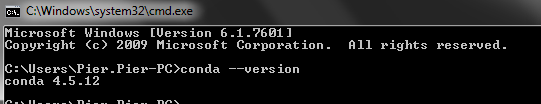
\includegraphics[scale=1]{figures/versiconda.png}
   	 \caption{Versi Anaconda Yang Digunakan}	
	\end{center}
\end{figure}
\item
Pastikan juga Kebutuhan Scikit seperti Numpy, Scipy dan Python telah terinstal. untuk mengeceknya buka CMD dan ketikan seperti gambar berikut.
\begin{figure}
	\begin{center}
   	 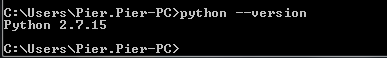
\includegraphics[scale=1]{figures/gambar.png}
   	 \caption{Versi Python Yang Digunakan}	
	\end{center}
\end{figure}
\item 
Pada CMD ketikan "conda install scikit-learn" kemudian tunggu sampai instalasi selesai.
\begin{figure}
	\begin{center}
   	 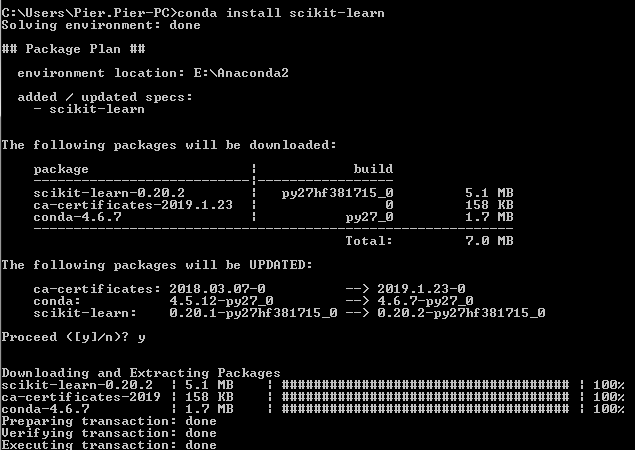
\includegraphics[scale=1]{figures/instalscikit.png}
   	 \caption{Instalasi Scikit Dari Anaconda}	
	\end{center}
\end{figure}
\item 
Setelah itu, kita akan mencoba salah satu contoh dasar penggunaan scikit pada website sebelumnya. Dan disini menggunakan contoh Multilabel classification.
\item 
Salin skrip contoh tersebut ke Text Editor Visual Code atau yang anda miliki. File ini kemudian di save dengan nama "contoh.py"
\begin{figure}
	\begin{center}
   	 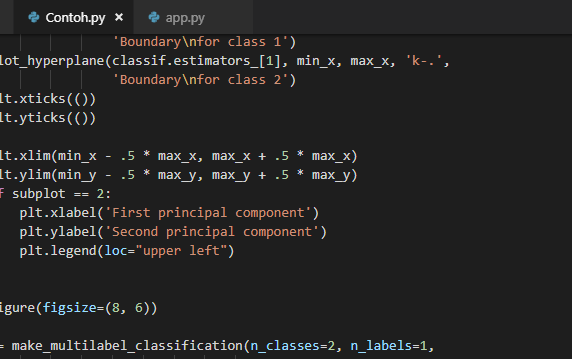
\includegraphics[scale=1]{figures/contoh.png}
   	 \caption{Contoh Skrip}	
	\end{center}
\end{figure}
\item 
Setelah tersimpan, jalankan di CMD dengan mengetikan "python contoh.py" maka akan muncul hasil seperti dibawah ini.
\begin{figure}
	\begin{center}
   	 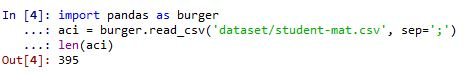
\includegraphics[scale=1]{figures/hasil1.png}
   	 \caption{Hasil Yang Muncul Di CMD}	
	\end{center}
\end{figure}
\begin{figure}
	\begin{center}
   	 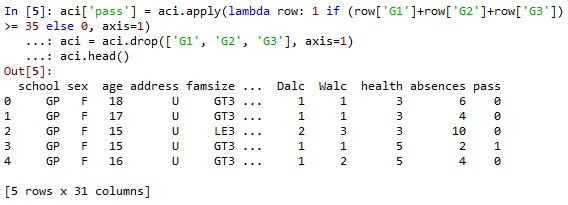
\includegraphics[scale=1]{figures/hasil2.png}
   	 \caption{Gambar Yang Muncul Dari Matplotlib}	
	\end{center}
\end{figure}
\end{enumerate}

\subsection{Mencoba Loading an example dataset, menjelaskan maksud dari tulisan tersebut dan mengartikan per baris}
\begin{enumerate}
\item
Mengimmport dataset, iris dan digit sebagai contoh data.
\begin{figure}
	\begin{center}
   	 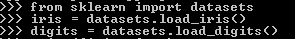
\includegraphics[scale=1]{figures/penjelasan1.png}
   	 \caption{Penjelasan }	
	\end{center}
\end{figure}
\item
Misalnya, dalam kasus dataset digit, digits.data memberikan akses ke fitur yang dapat digunakan untuk mengklasifikasikan sampel digit.
\begin{figure}
	\begin{center}
   	 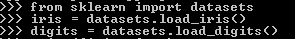
\includegraphics[scale=1]{figures/penjelasan1.png}
   	 \caption{Penjelasan 2}	
	\end{center}
\end{figure}
\item 
digit.target memberikan kebenaran dasar untuk dataset digit, yaitu angka yang sesuai dengan setiap gambar digit yang dipelajari.
\begin{figure}
	\begin{center}
   	 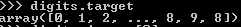
\includegraphics[scale=1]{figures/penjelasan3.png}
   	 \caption{Penjelasan 3}	
	\end{center}
\end{figure}
\item 
menggambarkan bagaimana mulai dari masalah awal seseorang dapat membentuk data untuk konsumsi di scikit-belajar.
\begin{figure}
	\begin{center}
   	 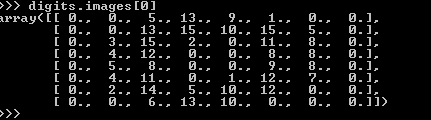
\includegraphics[scale=1]{figures/penjelasan4.png}
   	 \caption{Penjelasan 4}	
	\end{center}
\end{figure}

\end{enumerate}

\begin{enumerate}
\item
Mencoba Learning and predicting, menjelaskan maksud dari tulisan tersebut dan mengartikan per baris[hari ke 2](10)
\item
mencoba Model persistence, menjelaskan maksud dari tulisan tersebut dan mengartikan per baris[hari ke 2](10)
\item 
Mencoba Conventions, menjelaskan maksud dari tulisan tersebut dan mengartikan per baris[hari ke 2](10)
\end{enumerate}


\section{Penanganan Error}
Dari percobaan yang dilakukan di atas, apabila mendapatkan error maka:

\begin{enumerate}
	\item
	skrinsut error[hari ke 2](10)
	\item
Tuliskan kode eror dan jenis errornya [hari ke 2](10)
	\item
Solusi pemecahan masalah error tersebut[hari ke 2](10)

\end{enumerate}

